
\documentclass[sigconf,nonacm]{acmart}
\usepackage{graphicx}
\usepackage{url}


%% up to 2 pages for distributing at SC19 and some other places to
%% have more number of answers

\def\Underline{\setbox0\hbox\bgroup\let\\\endUnderline}
\def\endUnderline{\vphantom{y}\egroup\smash{\underline{\box0}}\\}
\def\|{\verb|}
%
\long\def\comment#1{}
%

\begin{document}

\title{Why do MPI users not use the state-of-the-art API?\\
- An Interim Report of MPI International Survey -}


\author{Atsushi Hori}
\email{ahori@riken.jp}
\author{Takashi Ogura}
\email{t-ogura@riken.jp}
\affiliation{\institution{R-CCS}}
 
\author{George Bosilca}
\email{bosilca@icl.utk.edu}
\affiliation{\institution{UTK/ICL}}
 
\author{Emmanuel Jeannot}
\email{emmanuel.jeannot@inria.fr}
\affiliation{\institution{Inria}}

\begin{abstract}
In 2017, ECP\cite{ECP} conducted a survey for MPI users in the ECP
project to reveal how MPI would/should be integrated with ECP
applications in the future\cite{osti_1462877}.  
We decided to conduct another MPI survey targeting MPI users in the
whole world. Since MPI is being widely-used vehicle for
high-performance computing, this relatively large-scale questionnaire 
survey would be beneficial not only for deciding the future direction
of MPI, but also the feature differences of MPI users among
countries and/or regions of the world.  Our survey is not only
international but also targeting from novice to expert users, unlike
the ECP survey.

This survey began from February of 2019 and more than 800 answers from
42 countries all over the world at the time of this writing.
Unfortunately some countries which are known to be very eager for HPC
has very little number of answers. So we decided not to close the
survey until we got enough number of answers from those
countries. This is the short interim report based the current answers
of the survey. 

In this short report, it is focused on which MPI aspects MPI users
mostly use and which ones do not. This survey reveals that many MPI
users do not use newly introduced MPI functions, such as PMPI, dynamic
process creation, and persistent communication. Other questions also
reveals that most MPI users learn MPI via Internet and/or some form of
online documents. Considering those results, a possible explanation is
that most MPI users miss the chance to learn MPI in a systematic way
and thus they are not aware of the newly introduced APIs.
\end{abstract}

\maketitle

\section{Questionnaire}

The points we kept in our mind while we were designing the
questions are; a) minimizing the number of questions, b) easy-to-answer,
c) avoiding ambiguity
The questionnaire is implemented by using Google Forms and Microsoft
Forms, and distributed
by sending e-mails to major mailing lists such as {\tt
  hpc-announce@mcs.anl.gov}. 
All data, a Python program to analyze the answers, and all reports
published so far (including this) are available from a GITHUB page
({\tt https://github.com/bosilca/MPIsurvey.git}).  

Table~\ref{tab:countries} shows the number of answers of top-10
countries. It should be noted that the question asked the
workplaces of participants for recent 5 years, not the nationality.
In this report, the countries and regions (a set of countries)
having more than 50 answers are considered as major countries to
compare regional differences.

{\small
\begin{table}[htb]%
\begin{center}%
\caption{\small Top 10 Countries}\label{tab:countries}%
\begin{tabular}{c|l|r}%
\hline%
Rank & Country & \# Answers \hspace{5mm} \\%
\hline%
1 & Germany 	& 159 \hspace{8mm} \\%
2 & France 	& 125 \hspace{8mm} \\%
3 & Russia 	& 94 \hspace{8mm} \\%
4 & UK 		& 64 \hspace{8mm} \\%
5 & Japan 	& 63 \hspace{8mm} \\%
6 & USA 		& 58 \hspace{8mm} \\%
6 & Italy 		& 57 \hspace{8mm} \\%
\hline
8 & Switzerland & 40 \hspace{8mm} \\%
9 & Korea, South & 27 \hspace{8mm} \\%
10 & Austria 	& 26 \hspace{8mm} \\%
\hline%
\multicolumn{3}{c}{42 countries, 838 participants} \\%
\end{tabular}%
\end{center}%
\end{table}%
}

Most answers, around 80\%, come from research organizations
(universities and governmental research institutes).  We do not think this
diversities did not reflect the characteristics of the countries, but
came from the biased questionnaire distribution. 
Since this profile may bias the analysis of the results, 
readers must keep this in their mind on this background.

\section{Some Results}

Table~\ref{tab:Q10-ans}, \ref{tab:Q14-ans}, \ref{tab:Q16-ans}, and
\ref{tab:Q17-ans} show the number of answers of 4 questions out of
30. Since those questions allow participants to choose multiple answers, 
the numbers in those tables are the numbers of answers of the
corresponding choices. The actual number of participants who answered
each question is noted after the slash (/) of the total number
at the end of each table.  

\begin{table*}[htb]%
%\footnotesize
\scriptsize
\begin{center}%
\begin{tabular}{c}

\begin{minipage}{0.24\hsize}
\begin{center}%
\caption{\small How did you learn MPI?}%
\label{tab:Q10-ans}%
\begin{tabular}{l|r}%
\hline%
Multiple Choice & \# Answers \\%
\hline%
Other lectures or tutorials & 436 (23.8\%) \\% 
Articles found on Internet & 430 (23.4\%) \\%
MPI standard doc. & 323 (17.6\%) \\% 
Lecture(s) at school & 292 (15.9\%) \\% 
Book(s) & 277 (15.1\%) \\%
Never learned MPI & 26 (1.4\%) \\%
other & 50 (2.7\%) \\%
\hline%
\multicolumn{1}{c}{total} & 1834 / 825 \\%
\hline%
\end{tabular}%
\end{center}%
\end{minipage}

\hspace{1mm}
\begin{minipage}{0.24\hsize}
\begin{center}%
\caption{\footnotesize How do you check MPI specifications when you are writing MPI programs?}%
\label{tab:Q14-ans}%
\begin{tabular}{l|r}%
\hline%
Multiple Choice & \# Answers \\%
\hline%
Online doc. & 570 (30.1\%) \\%
Internet & 560 (29.6\%) \\%
MPI standard doc. & 424 (22.4\%) \\%
I ask colleagues & 185 (9.8\%) \\%
I read book(s) & 102 (5.4\%) \\%
I know all MPI routines & 43 (2.3\%) \\%
other & 11 (0.6\%) \\%
\hline%
\multicolumn{1}{c}{total} & 1895 /824 \\%
\hline%
\end{tabular}%
\end{center}%
\end{minipage}

\hspace{1mm}
\begin{minipage}{0.24\hsize}
\begin{center}
\caption{\small Which MPI features have you never heard of?}%
\label{tab:Q16-ans}%
\begin{tabular}{l|r}%
\hline%
Multiple Choice & \# Answers \\%
\hline%
PMPI interface & 457 (24.5\%) \\%
Persistent comm. & 423 (22.7\%) \\%
Dynamic process creation & 380 (20.4\%) \\%
One-sided comm. & 128 (6.9\%) \\%
Communicator operations & 123 (6.6\%) \\%
MPI datatypes & 90 (4.8\%) \\%
Point-to-point comm. & 89 (4.8\%) \\%
Collective comm. & 86 (4.6\%) \\%
w/ OpenMP (multithread) & 86 (4.6\%) \\%
\hline%
\multicolumn{1}{c}{total} & 1,862 / 691 \\%
\hline%
\end{tabular}%
\end{center}%
\end{minipage}

\hspace{1mm}
\begin{minipage}{0.24\hsize}
\begin{center}
\caption{\footnotesize What aspects of the MPI standard do you use in your program in its current form?}%
\label{tab:Q17-ans}%
\begin{tabular}{l|r}%
\hline%
Multiple Choice & \# Answers \\%
\hline%
Collective comm. & 729 (22.5\%) \\%
Point-to-point comm. & 701 (21.6\%) \\%
MPI datatypes & 512 (15.8\%) \\%
w/ OpenMP (multithread) & 472 (14.6\%) \\%
Communicator operations & 406 (12.5\%) \\%
One-sided comm. & 223 (6.9\%) \\%
PMPI interface & 66 (2.0\%) \\%
Persistent comm. & 61 (1.9\%) \\%
Dynamic process creation & 50 (1.5\%) \\%
other & 20 (0.6\%) \\%
\hline%
\multicolumn{1}{c}{total} & 3,240 / 813 \\%
\hline%
\end{tabular}%
\end{center}
\end{minipage}

\end{tabular}%
\end{center}%
\end{table*}%

Table~\ref{tab:Q10-ans} shows the result of the question asking ``how
did you learn MPI.'' It is a bit surprising that 40\% (323/825) of
participants refer to the MPI standard. According to the original
data (omitted due to the space limit), one quarter of participants
learn MPI via the internet and/or online documents. 

The result of the question asking ``how do you check MPI
specifications when you are writing MPI programs'' is shown in
Table~\ref{tab:Q14-ans}. More than half of participants refer to the
MPI standard. It is very natural for MPI users to check MPI
specification by referring the MPI standard more often than reading it
for learning. Most notably, the percentage of participants reading
online documents and/or referring the internet occupies 46\% (original
data). 

Referring Table~\ref{tab:Q16-ans} and \ref{tab:Q17-ans}, The MPI
features can be categorized into two groups; well-known ones (P2P,
Collectives, and so on) and little-known ones (PMPI, Persistent and
Dynamic process). Surprisingly this tendency is almost independent
from countries/regions of the participants (Figure\ref{fig:Q17}). 

\comment{
Table~\ref{tab:Q16-ans} shows the answers of the question asking
``which MPI features have you never heard of?'' The answers of ``PMPI
interface,'' and ``Persistent communication,'' and ``Dynamic process
creation'' occupies almost 70\%.  The percentage of participants chose
one or some of them is 64\%.  
Table~\ref{tab:Q17-ans} shows the answers of the question asking
``what aspects of the MPI standard do you use in your program in its
current form?'' This question asks the MPI features used by
participants, not if they know or not. Again, there are large gap
between those three features and the other features.
All those features was already standardized in MPI 2.2 which was
release in 2009. Despite the 10-year appearance, those features are
not well-known. 
It is very interesting that the regional differences of the answers
asking which MPI features participants are using
(Table~\ref{tab:Q17-ans}) are very small as shown in
Figure~\ref{fig:Q17}. 
}

\begin{figure}[htb]
\begin{center}
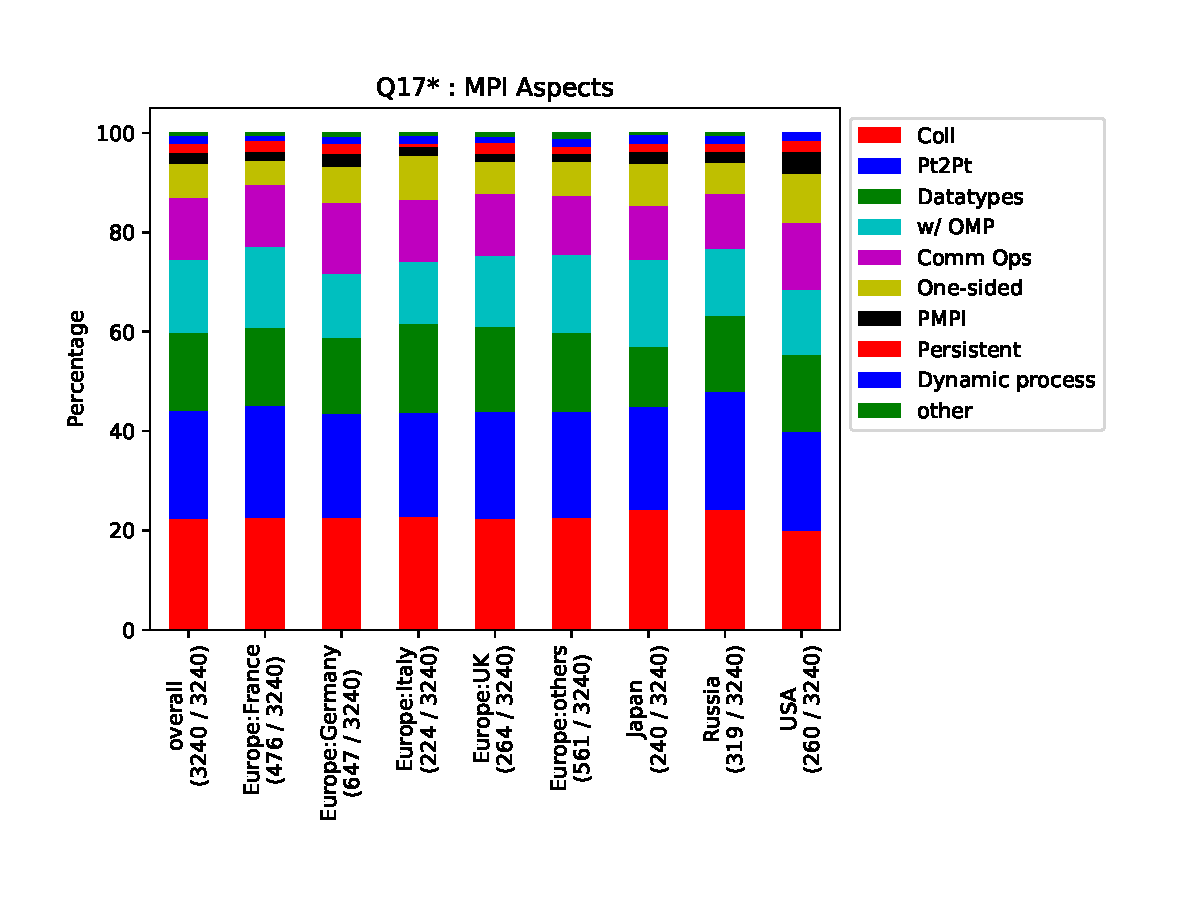
\includegraphics[width=8cm]{figs/Q17.pdf}
\vspace{-8mm}
\caption{What aspects of the MPI standard do you use in your program in its current form?}%
\label{fig:Q17}
\end{center}
\end{figure}

\comment{
On the question asking ``how did you learn MPI?,'' one quater of
participants answered ``internet,'' ``not learned,'' and ``other.'' Many
participants who chose ``other'' said ``learned from existing
code,''  ``learned by doing,'' etc. 
\comment{Table~\ref{tab:Q14-ans} shows the result of asking ``how do you check
MPI specifications when you are writing MPI programs?'' }
When we ask ``how do you check
MPI specifications when you are writing MPI programs?,'' 45\% of
participants chose the answers only from ``Online Docs,''
``Internet,'' and ``Asking colleagues.''
30\% of participants chose ``too many routines,'' ``too complicated,''
and/or ``I have nobody to ask,'' when the question ``what are your
obstacles to mastering MPI?'' was given. 
}
\comment{
\begin{table}[htb]%
\begin{center}%
\small
\caption{How do you check MPI specifications when you are writing MPI programs?}%
\label{tab:Q14-ans}%
\begin{tabular}{l|r}%
\hline%
Multiple Choice & \# Answers \\%
\hline%
{\small I read online documents (such as man pages).} & 570 (30.1\%) \\%
{\small I search the Internet} & 560 (29.6\%) \\%
{\small I read the MPI Standard document}  & 424 (22.4\%) \\%
I ask colleagues. & 185 (9.8\%) \\%
{\small I read book(s) (except the MPI standard).} & 102 (5.4\%) \\%
I know almost all MPI routines. & 43 (2.3\%) \\%
other & 11 (0.6\%) \\%
\hline%
\multicolumn{1}{c}{total} & 1,895 / 824 \\%
\hline%
\end{tabular}%
\end{center}%
\end{table}%
}

\section{MPI users do not use the state-of-the-art API}

Among the little-known MPI features, the persistent communication is
one of the important directions being discussed in MPI Forum\cite{mpi-forum}.
The persistent communication can give implementors a room for
optimization not only P2P but also collective communication
performance. 
All those little-known MPI features already appeared in MPI 2.2
released in 2009. Despite the 10-year appearance, those features 
are failed to get widely accepted. Why this happens?

One possible answer for this question may come from the survey results
asking participants ``how did you learn MPI''
(Table~\ref{tab:Q10-ans}) and ``how do you check
MPI specifications when you are writing MPI programs''
(Table~\ref{tab:Q14-ans}). 
Here a significant number of participants refer to internet
and/or online documents. These are handy and able to get required
information on the fly. However, 
these online medias can only be accessed by
search. To search something, a clue or some keywords must be given. 
Someone wants to search something he/she does not know, how can he/she
find the appropriate key words to obtain the right information? In
MPI, for example, there is no {\tt See Also} link from the man page of {\tt
  MPI\_Irecv}  to the corresponding persistent routines in many MPI
implementations. 

Contrastingly traditional medias such as books, lectures, and tutorials can be
systematic and complete, but not handy.  Once you learned MPI via some
of those traditional medias, you may feel that you already know
MPI. Unfortunately MPI standard keeps changing. It is very hard to
keep your knowledge up-to-date, especially MPI is not your major
concern. 

Another point we noticed is that many people who chose the ``other''
answer to the question asking ``how did you learn MPI'' said
``reading existing code,'' ``learn by doing,'' ``reverse
engineering''(!),  and so on. Taking a look at existing code might be
the way of learning programing nowadays. However, the underlying
rationale of every MPI feature is never simpler than any other
sequential programs and there are many possible pitfalls. 

\comment{
The traditional learning method, such as reading
books and/or having lectures, becomes less significant but this is the way
we have done so far. The learning-by-search can never be systematic and
learner may fall in pit-falls. The underlying rationale of every MPI
feature is never simpler than any other sequential programs. 
Thus, newly introduced features are hard to be widespread. 
}

\section{Summary}

As of this writing, we got only 8 answers from China. This is because 
Chinese government does not allow its people to access Google. We are
trying to increase the number of participants from the
countries which are aggressive in HPC.  
If some of readers are interested in participating this survey, visit
one (not both) of the URLs in Figure~\ref{fig:qrcodes}.

\begin{figure}[htb]
\begin{center}

\includegraphics[width=4cm]{figs/QR-codes.pdf}
\caption{QR codes to participate this survey}
\label{fig:qrcodes}
\end{center}
\end{figure}

\section*{Acknowledgment}
  We thank to those who participated in this survey and those who
  helped us to distribute the survey to their local communities.\\
  This research is partially supported by the
  NCSA-Inria-ANL-BSC-JSC-Riken-UTK Joint-Laboratory for Extreme Scale
  Computing\cite{JLESC}.

\bibliographystyle{acm}
\bibliography{../ref}

\end{document}
